Data-intensive workloads represent a significant portion of today's large-scale computation. The applications range from business intelligence, bioinformatics, recommendation, to data streaming from large-scale simulations, distributed sensors, and social networks. To speed up next-generation scientific discoveries or to maximize commercial profits, many applications require that the data are processed in nearly real-time. 

Parallel computing frameworks, such as MapReduce, Dryad, and Spark, have been widely adopted for large-scale data analytics and batched stream processing~\cite{Dean2004,Isard2007,Zaharia180560,Bhatotia2011}. To efficiently handle the sheer amounts of data and simultaneously utilize a cluster of nodes and/or multiple cores within a node, these frameworks typically arrange a job into hundreds or thousands of tasks scheduled to execute in parallel, each processing one partition of the whole dataset\footnote{For iterative and graph algorithms, multiple stages of such parallel execution may be needed.}. This paradigm is depicted in Figure~\ref{fig:engine}.

\begin{figure}[!t]
  \begin{center}
      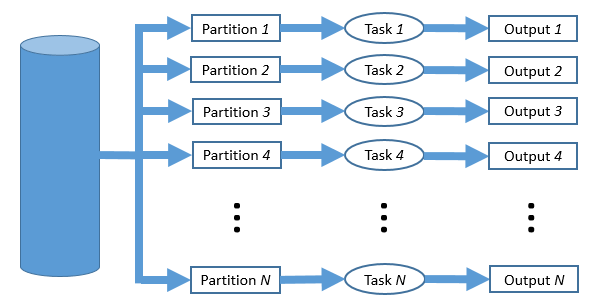
\includegraphics[width=\columnwidth]{figures/engine}
  \end{center}
  \vskip -0.1in
  \caption{Parallel data processing paradigm.}
  \label{fig:engine}
  %\vspace{-0.05in}
\end{figure}

The increasingly large scale of the HPC systems points to the growing interest in fault tolerance capability. There are a number of different causes of faults in computing systems. Faults can be attributed to both hardware, such as manufacture defects and wear-down, and software, including bugs, race-condition, and deadlocks. Additionally, system overloading can also lead to unexpected behaviors, e.g., a low priority job may be terminated to accommodate a high priority job. Despite the cause, fault can be classified into two types based on its externally visible manifestation: 1) crash failure, which forces the target processor to stop immediately; 2) silent data corruption, which allows the target processor to continue execution but produce incorrect results.  

In today's parallel computing frameworks, re-execution on top of a heartbeat protocol is mainly used to provide fault tolerance and to deal with staggers. This approach works fine for system scales such that failures are rare and applications that are delay-tolerant. If failures are frequent, however, large delay can be incurred since one faulty task or stagger may delay the whole job execution. In addition, re-execution only handles crash failures. This is not acceptable for applications with strict response time requirements or vulnerable to silent data corruption. In contrast, Shadow Computing, if applied, will enable these frameworks to trade-off among multiple objectives, while respecting any hard or soft deadline and handling both types of failures. 

%For the development of analytical models and optimization frameworks in the following sections, we define necessary notations here. 